\documentclass{standalone}
\usepackage{tikz}
\usetikzlibrary{shapes,arrows, positioning,matrix,calc}

\hyphenpenalty=10000
% https://texample.net/tikz/examples/simple-flow-chart/
% Define block styles
\tikzstyle{block} = [rectangle, draw, fill=blue!20, text centered, minimum height=1cm, outer sep=0pt, inner sep=0pt, anchor=north west]

\begin{document}
 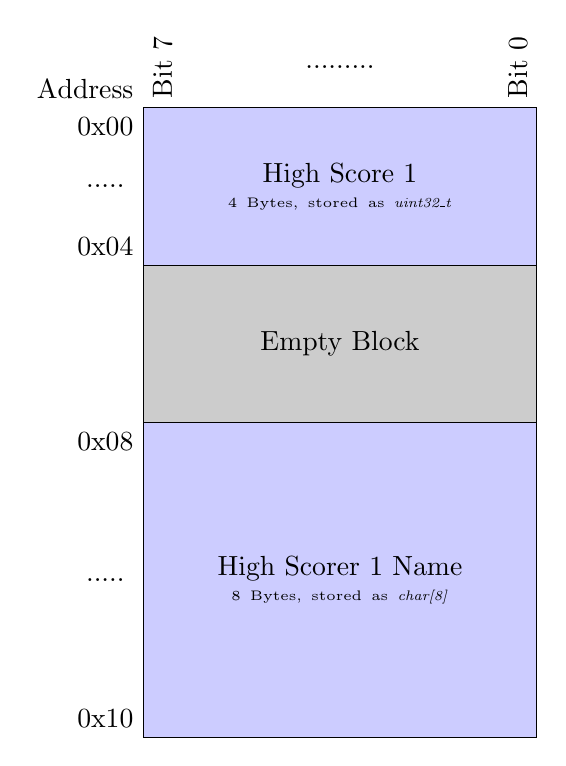
\begin{tikzpicture}[node distance=0cm]
    \renewcommand{\baselinestretch}{0.75}
    \node[block, text width=5cm, minimum height=2cm] (r1) at (0,0) {High Score 1\\\tiny{4 Bytes, stored as \textit{uint32\_t}}};
    \node[block, text width=5cm, minimum height=2cm, fill=black!20] (empty1) at (0,-2) {Empty Block};
    \node[block, text width=5cm, minimum height=4cm] (r2) at (0,-4)  {High Scorer 1 Name\\\tiny{8 Bytes, stored as \textit{char[8]}}};
    
    \node[left=of r1.north west, anchor=north east] (txt1) {0x00};
    \node[left=of r1.south west, anchor=south east] (txt2) {0x04};
    \node[] at ($(txt1)!0.5!(txt2)$) {.....};
    
    \node[left=of r2.north west, anchor=north east] (txt1) {0x08};
    \node[left=of r2.south west, anchor=south east] (txt2) {0x10};
    \node[] at ($(txt1)!0.5!(txt2)$) {.....};

 
    \node[above=of r1.north west, anchor=north west, rotate=90] (b7) {Bit 7};
    \node[above=of r1.north east, anchor=south west, rotate=90] (b0) {Bit 0};
    \node[] at ($(b7)!0.5!(b0)$) {.........};

    \node[anchor=south east] at(0,0) {Address};
 \end{tikzpicture}
\end{document}
